\documentclass[../notes.tex]{subfiles}

\pagestyle{main}
\renewcommand{\chaptermark}[1]{\markboth{\chaptername\ \thechapter\ (#1)}{}}
\setcounter{chapter}{7}

\begin{document}




\chapter{Many-Body Systems}
\section{The Many-Body Problem}
\begin{itemize}
    \item \marginnote{11/1:}Announcements.
    \begin{itemize}
        \item Exam room locations are on Canvas.
        \item Notice that we skipped \textcite{bib:KibbleBerkshire}, Chapter 6.
    \end{itemize}
    \item Recap: 2-body systems.
    \begin{itemize}
        \item In such a system, we have two particles: $m_1,\vec{r}_1$ and $m_2,\vec{r}_2$. Their mass sum is $M=m_1+m_2$, their center of mass is at $\vec{R}=(m_1\vec{r}_1+m_2\vec{r}_2)/(m_1+m_2)$, their reduced mass is $\mu=m_1m_2/(m_1+m_2)$, and their relative position is $\vec{r}=\vec{r}_1-\vec{r}_2$.
        \item Under a constant external force, their EOMs uncouple into $M\ddot{R}_i=Mg_i$ and $\mu\ddot{r}_i=-\pdv*{V_\text{int}}{r_i}$ where $V_\text{int}(\vec{r})$ is the interaction potential energy.
    \end{itemize}
    \item A better answer to last time's question, "what is the reduced mass?"
    \begin{itemize}
        \item Let's look at two important cases to start.
        \begin{enumerate}
            \item If $m_1=m_2$, $\mu=m_1/2=m_2/2$ and the particles are maximally affecting each other.
            \item If $m_1\ll m_2$, then
            \begin{equation*}
                \mu = \frac{m_1m_2}{m_2(1+m_1/m_2)}
                \approx m_1\left( 1-\frac{m_1}{m_2} \right)+\text{H.O.T.}
                \to m_1
            \end{equation*}
            where H.O.T. stands for "higher order terms."
        \end{enumerate}
        \item We now elaborate further on the second case above.
        \item Essentially, as $m_1/m_2\to 0$, we have
        \begin{align*}
            M &\to m_2&
            \mu &\to m_1&
            \vec{R} &\to \vec{r}_2&
            \vec{r}_2{}^* &\to 0&
            \vec{r} &\to \vec{r}_1{}^*
        \end{align*}
        \begin{itemize}
            \item Essentially, we approach the limit of 1 body orbiting a fixed object.
            \item This justifies the approximation made in earlier chapters of the Earth orbiting a fixed sun or a satellite orbiting the fixed Earth or more.
        \end{itemize}
    \end{itemize}
    \item This concludes our discussion of two-body systems.
    \item Today: Many-body systems.
    \begin{itemize}
        \item Lagrangian, CM frame.
        \item Rockets.
    \end{itemize}
    \item Let our $N$ particles be indexed by $\alpha=1,\dots,N$.
    \begin{itemize}
        \item Note that \textcite{bib:KibbleBerkshire} uses a different notation! They just say $\vec{r}_i$.
    \end{itemize}
    \item Under this notation\dots
    \begin{itemize}
        \item The mass sum is
        \begin{equation*}
            M = \sum_\alpha m_\alpha
        \end{equation*}
        \item The center of mass is
        \begin{equation*}
            \vec{R} = \frac{1}{M}\sum_\alpha m_\alpha\vec{r}_\alpha
        \end{equation*}
        \item The linear momentum is
        \begin{equation*}
            \vec{P} = \sum_\alpha m_\alpha\dot{\vec{r}}_\alpha
            = M\dot{\vec{R}}
        \end{equation*}
    \end{itemize}
    \item In the CM frame (still denoted $*$), we have
    \begin{equation*}
        \vec{r}_\alpha = \vec{R}+\vec{r}_\alpha{}^*
    \end{equation*}
    \begin{itemize}
        \item Moreover, within the frame, we still have $\dot{\vec{R}}{}^*=0$ and hence $\vec{P}{\,}^*=0$.
    \end{itemize}
    \item Using the above, we may define the kinetic energy for the system as
    \begin{align*}
        T &= \frac{1}{2}\sum_\alpha m_\alpha\dot{\vec{r}}_\alpha{}^2\\
        &= \frac{1}{2}\sum_\alpha m_\alpha(\dot{\vec{R}}+\dot{\vec{r}}_\alpha{}^*)^2\\
        &= \frac{1}{2}\Bigg( \dot{\vec{R}}{\,}^2\underbrace{\sum_\alpha m_\alpha}_M+2\dot{\vec{R}}\cdot\underbrace{\sum_\alpha m_\alpha\dot{\vec{r}}_\alpha{}^*}_{\substack{\vec{P}{\,}^*\\(=\,0)}}+\sum_\alpha m_\alpha(\dot{\vec{r}}_\alpha{}^*)^2 \Bigg)\\
        &= \frac{1}{2}M\dot{\vec{R}}{\,}^2+\frac{1}{2}\sum_\alpha m_\alpha(\dot{\vec{r}}_\alpha{}^*)^2\\
        &= T_\text{CM}+T^*
    \end{align*}
    \item We may now define the Lagrangian for the system.
    \begin{itemize}
        \item The kinetic energy $T$ is defined above.
        \item The potential energy $V$ is given by the following, where $\{\vec{r}_\alpha-\vec{r}_\beta\}$ denotes the vector with all pairwise differences.
        \begin{align*}
            V &= -\sum_\alpha m_\alpha\vec{r}_\alpha\cdot\vec{g}+V_\text{int}(\{\vec{r}_\alpha-\vec{r}_\beta\})\\
            &= -M\vec{g}\cdot\vec{R}+V_\text{int}(\{\vec{r}_\alpha-\vec{r}_\beta\})
        \end{align*}
        \item Therefore, the Lagrangian $L$ is given by
        \begin{align*}
            L &= T-V\\
            &= \frac{1}{2}M\dot{\vec{R}}{\,}^2+M\vec{g}\cdot\vec{R}+\frac{1}{2}\sum_\alpha m_\alpha(\dot{\vec{r}}_\alpha{}^*)^2-V_\text{int}(\{\vec{r}_\alpha-\vec{r}_\beta\})
        \end{align*}
    \end{itemize}
    \item Thus, the EOMs separate into the $1+3N$ following equations, where each of the $N$ $\alpha$'s have three components indexed by $i=q_1,q_2,q_3$ corresponding to the Cartesian directions.
    \begin{align*}
        M\ddot{\vec{R}} &= M\vec{g}&
        m_\alpha\ddot{r}_{\alpha_i}{}^* &= -\pdv{V_\text{int}}{r_{\alpha_i}{}^*}
    \end{align*}
    \item Moreover, we get two conservation laws.
    \begin{align*}
        \frac{1}{2}M\dot{\vec{R}}{\,}^2-M\vec{g}\cdot\vec{R} &= E&
        T^*+V_\text{int} &= E_\text{int}
    \end{align*}
    \item In the more general case wherein other forces act on the system, we have
    \begin{equation*}
        m_\alpha\ddot{\vec{r}}_\alpha = \sum_\beta\vec{F}_{\alpha\beta}+\vec{F}_\alpha
    \end{equation*}
    \begin{itemize}
        \item The $\vec{F}_{\alpha\beta}$ are internal pairwise forces.
        \item The singular $\vec{F}_\alpha$ represents an external force.
        \item Linear momentum in this case.
        \begin{align*}
            \dot{\vec{P}} &= \sum_\alpha m_\alpha\ddot{\vec{r}}_\alpha\\
            &= \sum_\alpha\sum_\beta\vec{F}_{\alpha\beta}+\sum_\alpha\vec{F}_\alpha
        \end{align*}
        \begin{itemize}
            \item Since $\vec{F}_{\alpha\beta}=-\vec{F}_{\beta\alpha}$, the left term above cancels, leaving us with
            \begin{equation*}
                \dot{\vec{P}} = \sum_\alpha\vec{F}_\alpha
                = M\ddot{\vec{R}}
            \end{equation*}
            \item Recall that if there are no external forces, $\vec{P}$ is constant.
        \end{itemize}
        \item Angular momentum in this case.
        \begin{equation*}
            \vec{J} = \sum_\alpha m_\alpha\vec{r}_\alpha\times\dot{\vec{r}}_\alpha
        \end{equation*}
        \begin{itemize}
            \item It follows that
            \begin{align*}
                \dot{\vec{J}} &= \sum_\alpha m_\alpha(\underbrace{\dot{\vec{r}}_\alpha\times\dot{\vec{r}}_\alpha}_0+\vec{r}_\alpha\times\ddot{\vec{r}}_\alpha)\\
                &= \sum_\alpha m_\alpha\vec{r}_\alpha\times\ddot{\vec{r}}_\alpha\\
                &= \sum_\alpha\vec{r}_\alpha\times(m_\alpha\ddot{\vec{r}}_\alpha)\\
                &= \sum_\alpha\vec{r}_\alpha\times\left( \sum_\beta\vec{F}_{\alpha\beta}+\vec{F}_\alpha \right)\\
                &= \sum_\alpha\vec{r}_\alpha\times\sum_\beta\vec{F}_{\alpha\beta}+\sum_\alpha\vec{r}_\alpha\times\vec{F}_\alpha\\
                &= \sum_\alpha\sum_\beta\vec{r}_\alpha\times\vec{F}_{\alpha\beta}+\sum_\alpha\vec{r}_\alpha\times\vec{F}_\alpha
            \end{align*}
            \begin{itemize}
                \item Note that $\dot{\vec{r}}_\alpha\times\dot{\vec{r}}=0$ because the cross product of any vector with itself is zero.
            \end{itemize}
            \item Now suppose that the $\vec{F}_{\alpha\beta}$ are central (i.e., parallel to $\vec{r}_\alpha-\vec{r}_\beta$). Then the left term in the last line of the preceding set of equations equals zero, as follows.
            \begin{align*}
                \sum_\alpha\sum_\beta\vec{r}_\alpha\times\vec{F}_{\alpha\beta} &= \sum_\alpha\vec{r}_\alpha\times\vec{F}_{\alpha\alpha}+\sum_{\alpha<\beta}(\vec{r}_\alpha\times\vec{F}_{\alpha\beta}+\vec{r}_\beta\times\vec{F}_{\beta\alpha})\\
                &= \sum_\alpha\vec{r}_\alpha\times 0+\sum_{\alpha<\beta}(\vec{r}_\alpha\times\vec{F}_{\alpha\beta}-\vec{r}_\beta\times\vec{F}_{\alpha\beta})\\
                &= \sum_\alpha 0+\sum_{\alpha<\beta}[(\vec{r}_\alpha-\vec{r}_\beta)\times\vec{F}_{\alpha\beta}]\\
                &= 0+\sum_{\alpha<\beta}0\\
                &= 0
            \end{align*}
            \item This leaves us with
            \begin{equation*}
                \dot{\vec{J}} = \sum_\alpha\vec{r}_\alpha\times\vec{F}_\alpha
            \end{equation*}
            i.e., $\dot{\vec{J}}$ is only affected by external forces in the central $\vec{F}_{\alpha\beta}$ case.
            \item Thus, if $\vec{F}_\alpha=0$, $\vec{J}$ is constant.
            \item Additionally, if $\vec{F}_\alpha$ are central, then $\vec{J}$ is constant because the cross product cancels.
        \end{itemize}
    \end{itemize}
    \item In the CM frame,
    \begin{equation*}
        \vec{J}{\,}^* = \sum_\alpha m_\alpha\vec{r}_\alpha{}^*\times\dot{\vec{r}}_\alpha{}^*
    \end{equation*}
    \begin{itemize}
        \item To relate this to the global angular momentum $\vec{J}$, first recall that $\vec{r}_\alpha=\vec{R}+\vec{r}_\alpha{}^*$. Then combine this equality with the original definition of angular momentum to yield
        \begin{align*}
            \vec{J} &= \sum_\alpha m_\alpha\vec{r}_\alpha\times\dot{\vec{r}}_\alpha\\
            &= \sum_\alpha m_\alpha(\vec{R}+\vec{r}_\alpha{}^*)\times(\dot{\vec{R}}+\dot{\vec{r}}_\alpha{}^*)\\
            &= \underbrace{\left( \sum_\alpha m_\alpha \right)}_M\vec{R}\times\dot{\vec{R}}+\underbrace{\left( \sum_\alpha m_\alpha\vec{r}_\alpha{}^* \right)}_{\substack{\vec{R}{\,}^*\\(=\,0)}}\times\dot{\vec{R}}+\vec{R}\times\underbrace{\left( \sum_\alpha m_\alpha\dot{\vec{r}}_\alpha{}^* \right)}_{\substack{\vec{P}{\,}^*\\(=\,0)}}+\sum_\alpha m_\alpha\vec{r}_\alpha{}^*\times\dot{\vec{r}}_\alpha{}^*\\
            &= M\vec{R}\times\dot{\vec{R}}+\vec{J}{\,}^*
        \end{align*}
        \item It follows since $\vec{r}_\alpha=\vec{R}+\vec{r}_\alpha{}^*$ once again that for central $\vec{F}_{\alpha\beta}$,
        \begin{align*}
            \dot{\vec{J}}{\,}^* &= \dot{\vec{J}}-\dv{t}(M\vec{R}\times\dot{\vec{R}})\\
            &= \dot{\vec{J}}-(M\dot{\vec{R}}\times\dot{\vec{R}}+M\vec{R}\times\ddot{\vec{R}})\\
            &= \dot{\vec{J}}-M\vec{R}\times\ddot{\vec{R}}\\
            &= \dot{\vec{J}}-\vec{R}\times\sum_\alpha\vec{F}_\alpha\\
            &= \sum_\alpha\vec{r}_\alpha\times\vec{F}_\alpha-\vec{R}\times\sum_\alpha\vec{F}_\alpha\\
            &= \sum_\alpha\vec{r}_\alpha{}^*\times\vec{F}_\alpha
        \end{align*}
    \end{itemize}
    \item An application of these multi-body systems: Rockets!
    \begin{itemize}
        \item Consider a rocket traveling forward at velocity $v$.
        \item To propel itself forward, it ejects mass $\dd{m}$ at a constant speed $u$ relative to the rocket.
        \item After the ejection, the mass $\dd{m}$ travels backwards at speed $v-u$ and the remaining rocket $M-\dd{m}$ travels forward at velocity $v+\dd{v}$.
        \item We have conservation of momentum in this "explosion," so
        \begin{align*}
            (M-\dd{m})(v+\dd{v})+\dd{m}(v-u) &= Mv\\
            Mv+M\dd{v}-v\dd{m}-\underbrace{\dd{m}\dd{v}}_0+v\dd{m}-u\dd{m} &= Mv\\
            M\dd{v} &= u\dd{m}\\
            &= -u\dd{M}\\
            \frac{\dd{v}}{u} &= -\frac{\dd{M}}{M}\\
            \frac{v}{u} &= -\ln\frac{M}{M_0}\\
            M &= M_0\e[-v/u]
        \end{align*}
    \end{itemize}
\end{itemize}



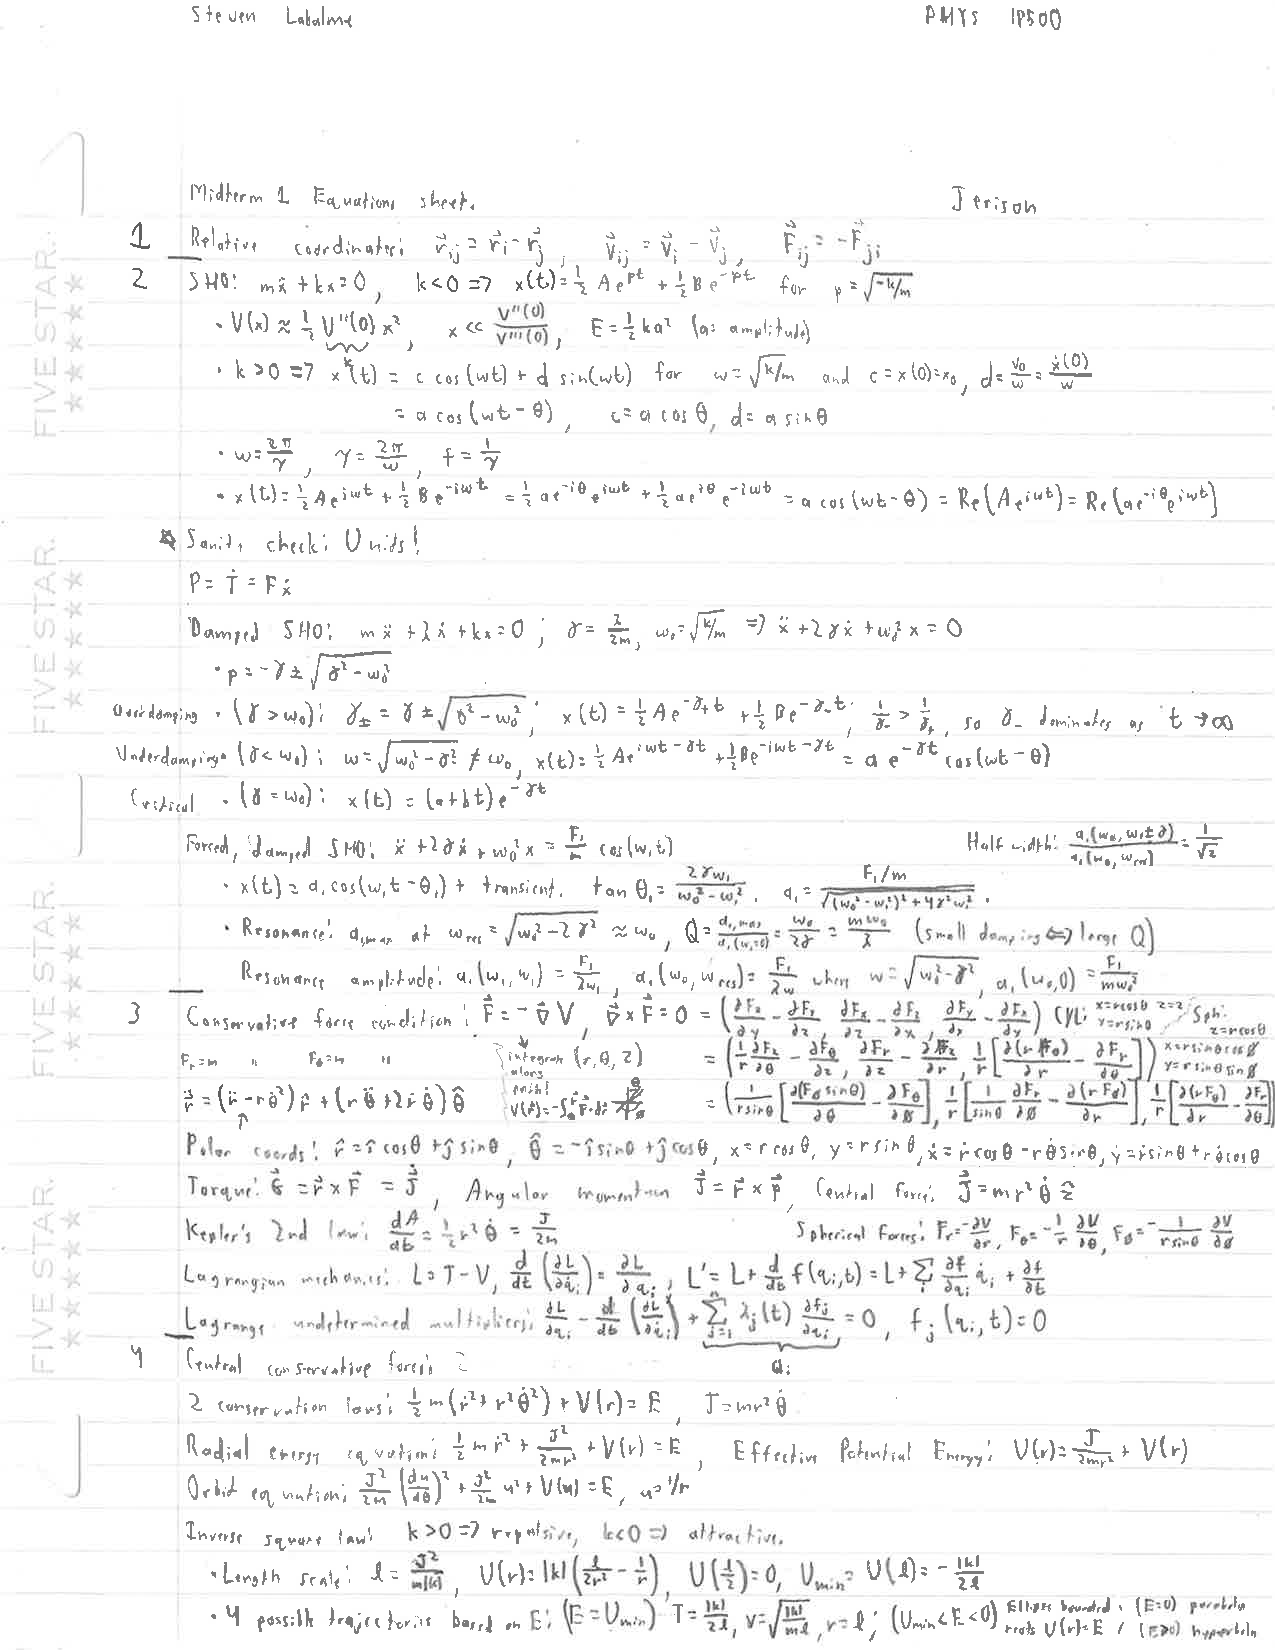
\includepdf[pages=-,addtotoc={1,section,1,Midterm 1 Equations Sheet,p1}]{../ExtFiles/Midterm1EqnSheet.pdf}



\section{Introduction; Rotation About an Axis; Moments of Inertia}
\begin{itemize}
    \item \marginnote{11/3:}Announcements.
    \begin{itemize}
        \item We will now have \emph{seven} problem sets instead of \emph{eight}.
        \begin{itemize}
            \item Each problem set is now worth more (PSets still amount to 40\% of our grade).
            \item There will still be one makeup PSet at the end of the quarter.
        \end{itemize}
        \item PSet 5 is due next Friday.
    \end{itemize}
    \item Recap: Many-body motion.
    \begin{itemize}
        \item It's useful to introduce the center of mass coordinate, $\vec{R}=1/M\cdot\sum_\alpha m_\alpha\vec{r}_\alpha$, where $M=\sum_\alpha m_\alpha$.
        \item In the CM frame, $\vec{R}{\,}^*=0$ and $\vec{r}_\alpha=\vec{R}+\vec{r}_\alpha{}^*$.
        \begin{itemize}
            \item We also have $\vec{P}{\,}^*=0$, $T^*=\sum_\alpha m_\alpha(\dot{\vec{r}}_\alpha{}^*)^2/2$, and $\vec{J}{\,}^*=\sum_\alpha m_\alpha\vec{r}_\alpha{}^*\times\dot{\vec{r}}_\alpha{}^*$.
        \end{itemize}
        \item Then, going back into the lab frame, we have $\vec{P}=M\cdot\dot{\vec{R}}$, $T=M\dot{\vec{R}}^2/2+T^*$, and $\vec{J}=M\vec{R}\times\dot{\vec{R}}+\vec{J}{\,}^*$.
    \end{itemize}
    \item One more note before we move onto rigid bodies: Suppose we're interested in the work, i.e., the rate of change of $T$ in the system.
    \begin{itemize}
        \item Recall that $m\ddot{\vec{r}}_\alpha=\sum_\beta\vec{F}_{\alpha\beta}+\vec{F}_\alpha$.
        \item Thus,
        \begin{align*}
            \dot{T} &= \dv{t}(\frac{1}{2}\sum_\alpha m_\alpha\dot{\vec{r}}_\alpha{}^2)\\
            &= \dv{t}(\frac{1}{2}\sum_\alpha m_\alpha\dot{\vec{r}}_\alpha\cdot\dot{\vec{r}}_\alpha)\\
            &= \frac{1}{2}\sum_\alpha m_\alpha(\ddot{\vec{r}}_\alpha\cdot\dot{\vec{r}}_\alpha+\dot{\vec{r}}_\alpha\cdot\ddot{\vec{r}}_\alpha)\\
            &= \frac{1}{2}\sum_\alpha 2m_\alpha\dot{\vec{r}}_\alpha\cdot\ddot{\vec{r}}_\alpha\\
            &= \sum_\alpha m_\alpha\dot{\vec{r}}_\alpha\cdot\ddot{\vec{r}}_\alpha\\
            &= \sum_\alpha\sum_\beta\dot{\vec{r}}_\alpha\cdot\vec{F}_{\alpha\beta}+\sum_\alpha\dot{\vec{r}}_\alpha\cdot\vec{F}_\alpha
        \end{align*}
        \item Note: At this point, we might naturally think that --- analogously to before --- the left term above will go to zero by letting $\vec{r}_{\alpha\beta}=\vec{r}_\alpha-\vec{r}_\beta$ and using $\vec{F}_{\alpha\beta}=-\vec{F}_{\beta\alpha}$.
        \begin{itemize}
            \item However, there is no reason for it to vanish this time.
            \item This should not be surprising since it makes sense that the internal potential energy of the system, which this term describes, would change in many cases.
        \end{itemize}
        \item Special case: If the $\vec{F}_{\alpha\beta}$ are conservative, then that rate at which the internal forces do work is
        \begin{align*}
            -\dv{t}V_{\text{int},\alpha\beta} &= -\dv{t}[V_{\text{int},\alpha\beta}(\vec{r}_\alpha-\vec{r}_\beta)]\\
            &= -\dv{(\vec{r}_\alpha-\vec{r}_\beta)}[V_{\text{int},\alpha\beta}(\vec{r}_\alpha-\vec{r}_\beta)]\cdot\dv{t}(\vec{r}_\alpha-\vec{r}_\beta)\\
            &= \vec{F}_{\alpha\beta}\cdot(\dot{\vec{r}}_\alpha-\dot{\vec{r}}_\beta)\\
            &= \vec{F}_{\alpha\beta}\cdot\dot{\vec{r}}_{\alpha\beta}\\
            &= \dot{\vec{r}}_{\alpha\beta}\cdot\vec{F}_{\alpha\beta}
        \end{align*}
        \begin{itemize}
            \item Consequence: The rate of change of the kinetic plus internal potential energy (i.e., total energy) is equal to the rate at which the external forces do work. That is,
            \begin{equation*}
                \dv{t}(T+V_\text{int}) = \sum_\alpha\dot{\vec{r}}_\alpha\cdot\vec{F}_\alpha
            \end{equation*}
        \end{itemize}
        \item Additionally, we can find the rate of change of energy relative to the center of mass.
        \begin{itemize}
            \item To begin, in the CM frame, we have
            \begin{equation*}
                \dv{t}(\frac{1}{2}M\dot{\vec{R}}^2) = M\dot{\vec{R}}\cdot\ddot{\vec{R}}
                = \dot{\vec{R}}\cdot\sum_\alpha\vec{F}_\alpha
            \end{equation*}
            \item Thus, subtracting the above equation from the one above it, we obtain
            \begin{align*}
                \dv{t}(T^*+V_\text{int}) &= \dv{t}(T-\frac{1}{2}M\dot{\vec{R}}^2+V_\text{int})\\
                &= \sum_\alpha\dot{\vec{r}}_\alpha\cdot\vec{F}_\alpha-\dot{\vec{R}}\cdot\sum_\alpha\vec{F}_\alpha\\
                &= \sum_\alpha\dot{\vec{r}}_\alpha{}^*\cdot\vec{F}_\alpha
            \end{align*}
        \end{itemize}
        \item Note that in the first term above, we are differentiating the total energy in the CM frame with respect to time. But since the time rate of change of energy is power, what we have expressed is the power.
    \end{itemize}
    \item Comparing this to $\dot{\vec{J}}{\,}^*=\sum_\alpha\vec{r}_\alpha{}^*\times\vec{F}_\alpha$, we see that we have a similar structure.
\end{itemize}



\section{Chapter 8: Many-Body Systems}
\emph{From \textcite{bib:KibbleBerkshire}.}
\begin{itemize}
    \item \marginnote{11/2:}Motivation: Studying material objects that can be regarded as "composed of a large number of small particles, small enough to be treated as essentially point-like but still large enough to obey the laws of classical rather than quantum mechanics. These particle interact in complicated ways with each other and with the environment. However, as we shall see, if we are interested only in the motion of the object as a whole, many of these details are irrelevant" \parencite[177]{bib:KibbleBerkshire}.
    \item We covered, line-for-line, Sections 8.1-8.2, and a good bit of 8.4-8.5.
    \item \marginnote{12/3:}EOMs of the $N$ particles.
    \begin{equation*}
        m_i\ddot{\vec{r}}_i = F_{i1}+\cdots+F_{iN}+F_i
        = \sum_jF_{ij}+F_i
    \end{equation*}
    \item Note that $F_{ii}=0$ for all $i=1,\dots,N$.
    \item Newton's three laws can be applied to composite bodies of $N$ particles as well as point particles.
    \begin{enumerate}
        \item If the body (that is, the system of $N$ particles) is \textbf{isolated}, it (that is, its center of mass) moves with uniform velocity.
        \item Interpreting the \emph{force} on the body to be the sum of the external forces on all of its constituent particles and the \emph{mass} of the body to be the sum of the masses of all of its constituent particles, we have as in class that
        \begin{equation*}
            \sum_i\vec{F}_i = M\ddot{\vec{R}}
        \end{equation*}
        \item Applies because it applies to each pair of particles from two composite bodies by generalizing them into one big body and reindexing.
    \end{enumerate}
    \item This discussion of finite collections of particles can easily be generalized to a continuous distribution of infinitesimal particles.
    \item Note that we may need some information about the shape of a body to calculate the total force acting on it.
    \begin{itemize}
        \item Example: A collection of particles in a non-uniform gravitational field; we need to know how far each particle is from the center of attraction.
    \end{itemize}
    \item A note on the rocket equation.
    \begin{itemize}
        \item The velocity of the rocket depends only on the ejection velocity and fraction of mass ejected, not the rate of ejection.
        \item Implication: In the absence of other forces, a brief and intense ejection provides as much thrust as a prolonged and gentle one.
        \item In the presence of other forces of course, such as gravity, a brief and intense ejection is necessary to overcome the constant retarding force.
    \end{itemize}
    \item \textbf{Velocity impulse}: The amount by which the velocity of a rocket changes under a thrust burst short enough for the change in position of the rocket during the burst to be negligible.
    \begin{itemize}
        \item "The relevant quantity for determining the mass of the rocket required to deliver a given payload, using a given ejection velocity, via a given orbital maneuver, is then the sum of the velocity impulses (in the ordinary, not the vector, sense)" \parencite[180]{bib:KibbleBerkshire}.
    \end{itemize}
    \item Elaborating on the compression of the internal angular momentum term.
    \begin{figure}[h!]
        \centering
        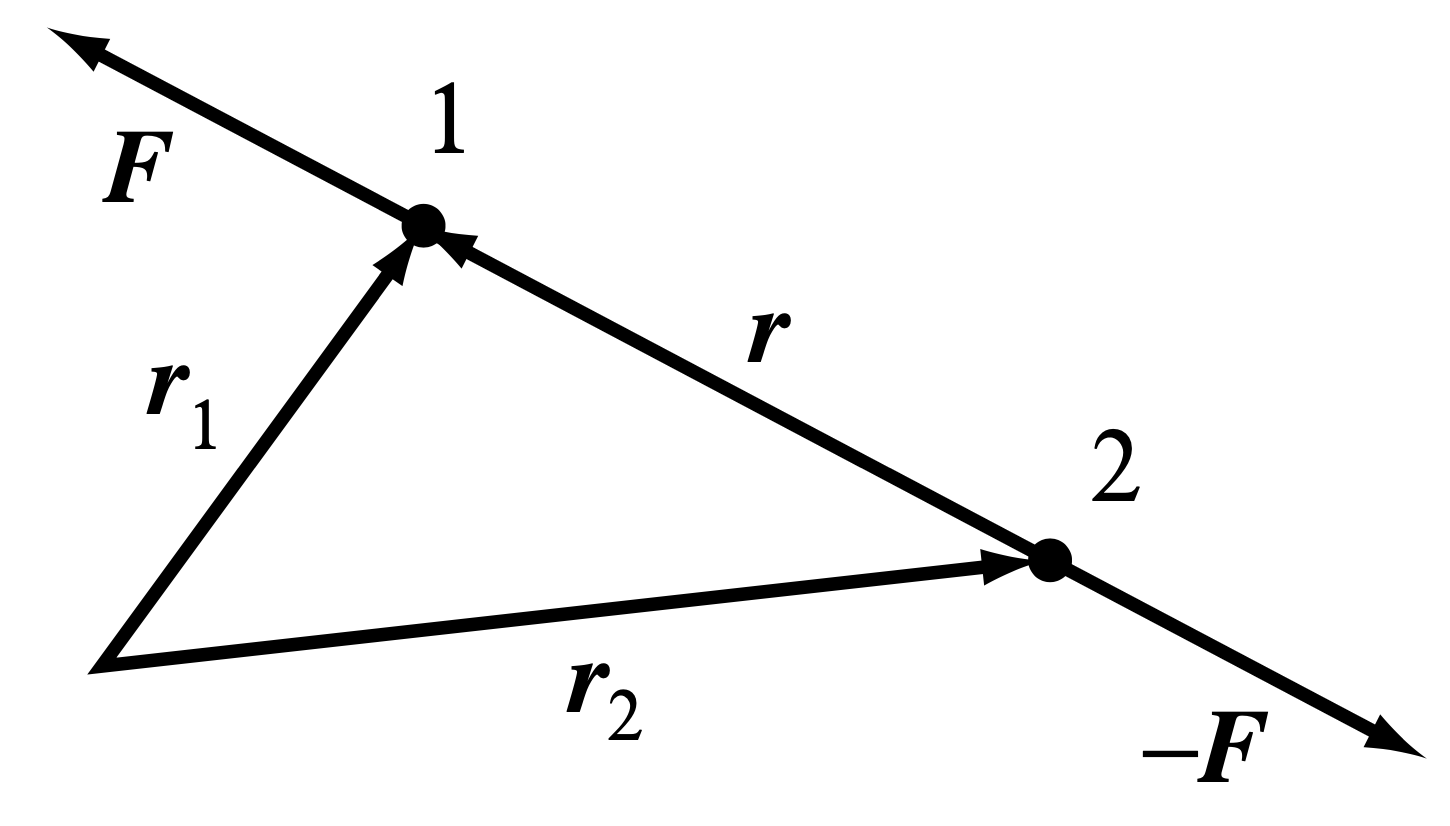
\includegraphics[width=0.25\linewidth]{../ExtFiles/manyBodAngMom.png}
        \caption{Internal forces and angular momentum.}
        \label{fig:manyBodAngMom}
    \end{figure}
    \begin{itemize}
        \item We have that
        \begin{equation*}
            \vec{r}_1\times\vec{F}_{12}+\vec{r}_2\times\vec{F}_{21} = \vec{r}_1\times\vec{F}-\vec{r}_2\times\vec{F}
            = \vec{r}\times\vec{F}
            = 0
        \end{equation*}
    \end{itemize}
    \item Generalizing the following results.
    \begin{equation*}
        \dot{\vec{J}}{\,}^* = \sum_\alpha\vec{r}_\alpha{}^*\times\vec{F}_\alpha
    \end{equation*}
    \begin{itemize}
        \item We may take moments about the origin of any \emph{inertial} frame.
        \item It would be wrong, however, to take moments about an \emph{accelerated} point unless the point in question is the center of mass (or in other very special cases).
        \item Implication: In discussing the rotational motion of a body, we can ignore the motion of its center of mass.
    \end{itemize}
    \item Consideration of the external potential energy, especially in the conservative case.
\end{itemize}




\end{document}